\documentclass{article}
\usepackage{nopageno}
\usepackage[utf8]{inputenc}

\usepackage{pdflscape}

\title{CLIN28 booklet}

\usepackage{textcomp}
\usepackage{url}
\usepackage{makecell}

\usepackage{array}

\usepackage{booktabs}
\usepackage{longtable}
\usepackage{pgfplotstable,filecontents}
\pgfplotsset{compat=1.9}

\newlength{\MyCellWidth}
\setlength{\MyCellWidth}{4cm}   % Saving fboxsep into mylength


\usepackage[a4paper, total={6in, 8in}]{geometry}
\geometry{textheight=750pt}
\setlength{\parindent}{0pt}

\usepackage{changepage}

\newcommand{\titloc}[2]{\begin{tabular}[t]{@{}p{\MyCellWidth}@{}}\textbf{#1}\\{}#2\end{tabular}}
\newcommand{\titloco}[2]{\begin{tabular}[t]{@{}l@{}}\textbf{#1}\\{}#2\end{tabular}}
\newcommand{\titaut}[2]{\begin{tabular}[t]{@{}p{\MyCellWidth}@{}}\textbf{#1} \\{}#2\end{tabular}}
\newcommand{\titautf}[2]{\hspace*{-0.1cm}\textit{#1}\begin{adjustwidth}{2cm}{}#2\end{adjustwidth}\leavevmode}

\usepackage{pgffor, ifthen}
\newcommand{\notes}[3][\empty]{%
    \noindent Notes\vspace{10pt}\\
    \foreach \n in {1,...,#2}{%
        \ifthenelse{\equal{#1}{\empty}}
            {\rule{#3}{0.5pt}\\}
            {\rule{#3}{0.5pt}\vspace{#1}\\}
        }
}

\usepackage{datatool}
\DTLsetseparator{;}

\DTLloaddb{posters}{posters.csv}
\DTLloaddb{presentations}{presentations.csv}

\usepackage{pdfpages}

\begin{document}

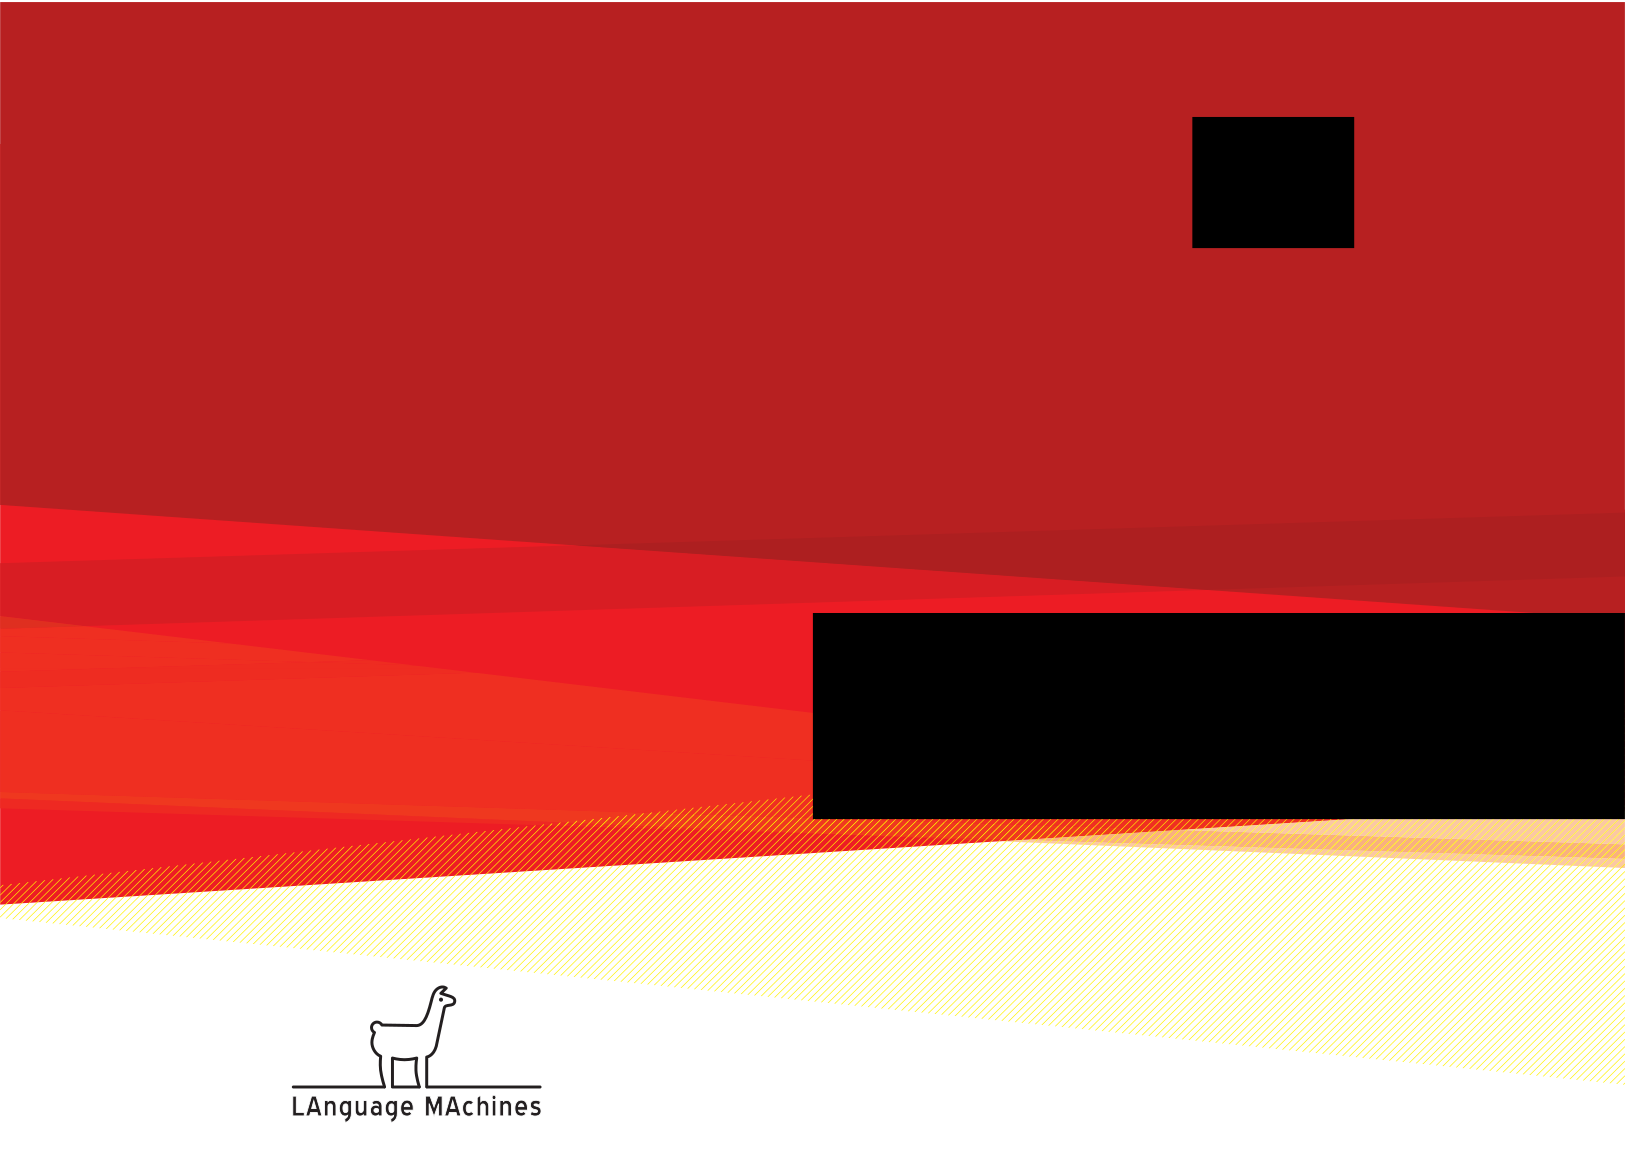
\includepdf[noautoscale, clip, trim=21.5cm 0cm 0.0cm 0.0cm, width=1.00\paperwidth]{front}
											\hspace{0pt}
\vspace{\fill}
\begin{center}
  {\Huge CLIN 28}\\[2em]

  Book of abstracts for the \\ 28th meeting of Computational Linguistics in the Netherlands \\[5cm]

  Nijmegen, 26 January 2018
\end{center}
\vspace{\fill}
\hspace{0pt}

\newpage	\hspace{0pt}
\vspace{\fill}

Automagically generated and typeset in \LaTeX. \\[2em]

Book of abstracts of the 28th Meeting of Computational Linguistics in the Netherlands (CLIN 28).\\[1em]

De Vereeniging, Nijmegen \\[2em]

\textcopyleft 2018
\url{https://github.com/LanguageMachines/clin28}

Book: louis \\
Font logo: Final Frontier Old Style by Allen R. Walden \\
Contact: \url{clin28@cls.ru.nl}
	\newpage	\section*{Preface}



Welcome to the 28th Computational Linguistics in The Netherlands meeting!\\[1em]

Yet again, CLIN, the non-centrally organised yearly meeting of computational linguists from the Low Countries, returns to Nijmegen, one of the pillars of computational linguistics in the Netherlands since the early 1970s. In large brushstrokes, Nijmegen was the home of Jan Aarts’ corpus linguistics group TOSCA, Jan van Bakel’s more formally oriented computational linguistics group, Gerard Kempen’s all-round cognitive and computational psycholinguistics group, Theo van den Heuvel’s Polderland, and Lou Boves’ speech technology group. Presently, work in computational linguistics and speech technology happens at the Centre for Language and Speech Technology (formerly SPEX) within the Faculty of Arts of Radboud University. This work echoes that of their predecessors: it is closely tied with speech technology research, and while being characterised mostly as data-driven and empirical, the research maintains strong ties to theoretical linguistics. Computational linguistics in Nijmegen continues to profit, furthermore, of the presence of  psycholinguistic and sociolinguistic expertise, a strong communication and information science group, and the on-campus research in artificial intelligence, data science, and more recently neuroscience.\\[1em]

Welcome to Nijmegen!\\[1em]

Concertgebouw De Vereeniging, the centrally located 1916 concert hall inviting architecture buffs to spot its Art Deco and Art Nouveau elements, offers the surroundings of this year’s CLIN. We are happy and proud to present prof.~Andy Way (Dublin City University) as keynote speaker who will talk about machine translation. It will be an interesting challenge for you, as usual, to find an optimal way through the interesting program with 44 oral presentations in four parallel sessions (one of which will be the winner of the STIL Master Thesis Prize) and 40 poster presentations.\\[1em]

Many thanks are due to the Centre for Language and Speech Technology and to our sponsors for their contribution to CLIN28, and to the organising team: Florian Kunneman, Iris Hendrickx, Merijn Beeksma, Frank Grootjen, Erkan Basar, Alessandro Lopopolo, Chara Tsoukala, Christoph Aurnhammer, Nelleke Oostdijk, Eric Sanders, Louis Onrust, Maarten van Gompel, and Hans van Halteren.\\[1em]

In the wake of CLIN28 a call for submissions will be sent to all contributors of accepted CLIN28 contributions for the 8th Volume of the CLIN Journal, which will publish a peer-reviewed selection of papers of this year’s CLIN. \\[1em]

Enjoy CLIN28!\\[1em]

Antal van den Bosch



\newpage	\subsection{Committees}


\subsubsection{Organising Committee}
Christoph Aurnhammer, M. Erkan Basar, Merijn Beeksma, Antal van den Bosch, Franc Grootjen, Iris Hendrickx, Florian Kunneman, Alessandro Lopopolo, louis onrust, Chara Tsoukala

\subsubsection{Support}
Maarten van Gompel, Hans van Halteren, Ian Hancock, Ali Hürriyetoglu, Yung Han Khoe, Ekaterina Slesareva, Eric Sanders, Odette Scharenborg, Ko van der Sloot, Tim Voets, Peter van de Water 


\subsection{Past, Present, and Future CLIN meetings}
\pgfplotstabletypeset[col sep=semicolon,
every head row/.style={output empty row},
     columns={Year,Date,Host},columns/Year/.style={string type},
    columns/Date/.style={string type,column type=l},
    columns/Host/.style={string type,column type=l},
    ]{clins.csv}
		\newpage	\section{Sponsors}

\subsection{Gold}
\begin{center}
    
\includegraphics[width=0.75\textwidth]{int-logo}
\end{center}

\subsection{Silver}
\begin{center}
    
\includegraphics[width=0.45\textwidth]{LI_logo_RGB_tag} \\[2cm]
    
\includegraphics[width=0.45\textwidth]{textkernel-tagline}
\end{center}

\subsection{Bronze}
\begin{center}
    
\includegraphics[width=0.3\textwidth]{logo_beeld_geluid} \hspace{2cm}
    
\includegraphics[width=0.3\textwidth]{logo_NOTaS} \\[2cm]
    
\includegraphics[width=0.3\textwidth]{logo_clariah} \hspace{2cm}
    
\includegraphics[width=0.3\textwidth]{siks-logo} \\[2cm]
    
\includegraphics[width=0.3\textwidth]{textgainlogo} \hspace{2cm}
    
\includegraphics[width=0.3\textwidth]{logoAG_XL}
\end{center}

\newpage						\newpage	\hspace{0pt}
\vspace{\fill}
\begin{center}
Programme
\end{center}
\vspace{\fill}
\hspace{0pt}

\newpage

\begin{landscape}
\pgfplotstabletypeset[begin table=\begin{longtable},
end table=\end{longtable},col sep=semicolon,
     columns={Time,S1,S2,S3,S4,S5},every head row/.style={ 
             output empty row},
             every row no 0/.style={after row=\midrule},
             every row no 5/.style={after row=\midrule},
             every row no 6/.style={after row=\midrule},
             every row no 7/.style={after row=\midrule},
             every row no 8/.style={after row=\midrule},
             every row no 9/.style={after row=\midrule},
             every row no 10/.style={after row=\midrule},
             every row no 11/.style={after row=\midrule},
             every row no 15/.style={after row=\midrule},
             every row no 16/.style={after row=\midrule},
             every row no 21/.style={after row=\midrule},
             every row no 22/.style={after row=\midrule},
    columns/Time/.style={string type,column type=p{\MyCellWidth}},
    columns/S1/.style={string type,column type=p{\MyCellWidth}},
    columns/S2/.style={string type,column type=p{\MyCellWidth}},
    columns/S3/.style={string type,column type=p{\MyCellWidth}},
    columns/S4/.style={string type,column type=p{\MyCellWidth}},
    columns/S5/.style={string type,column type=p{\MyCellWidth}},
    ]{schedule.csv} 
\end{landscape}

\newpage

\subsection{Keynote}

\subsection{Oral presentations}

\DTLsort{Title=ascending}{presentations}
\DTLforeach*%
{presentations}% database label
{\name=Title,\points=Authors}% assignment
{% Stuff to do at each iteration:
\titautf{\name}{\points}
}

\subsection{Posters}

\DTLsort{Title=ascending}{posters}
\DTLforeach*%
{posters}% database label
{\name=Title,\points=Authors}% assignment
{% Stuff to do at each iteration:
\titautf{\name}{\points}
}



\newpage

\begin{landscape}
    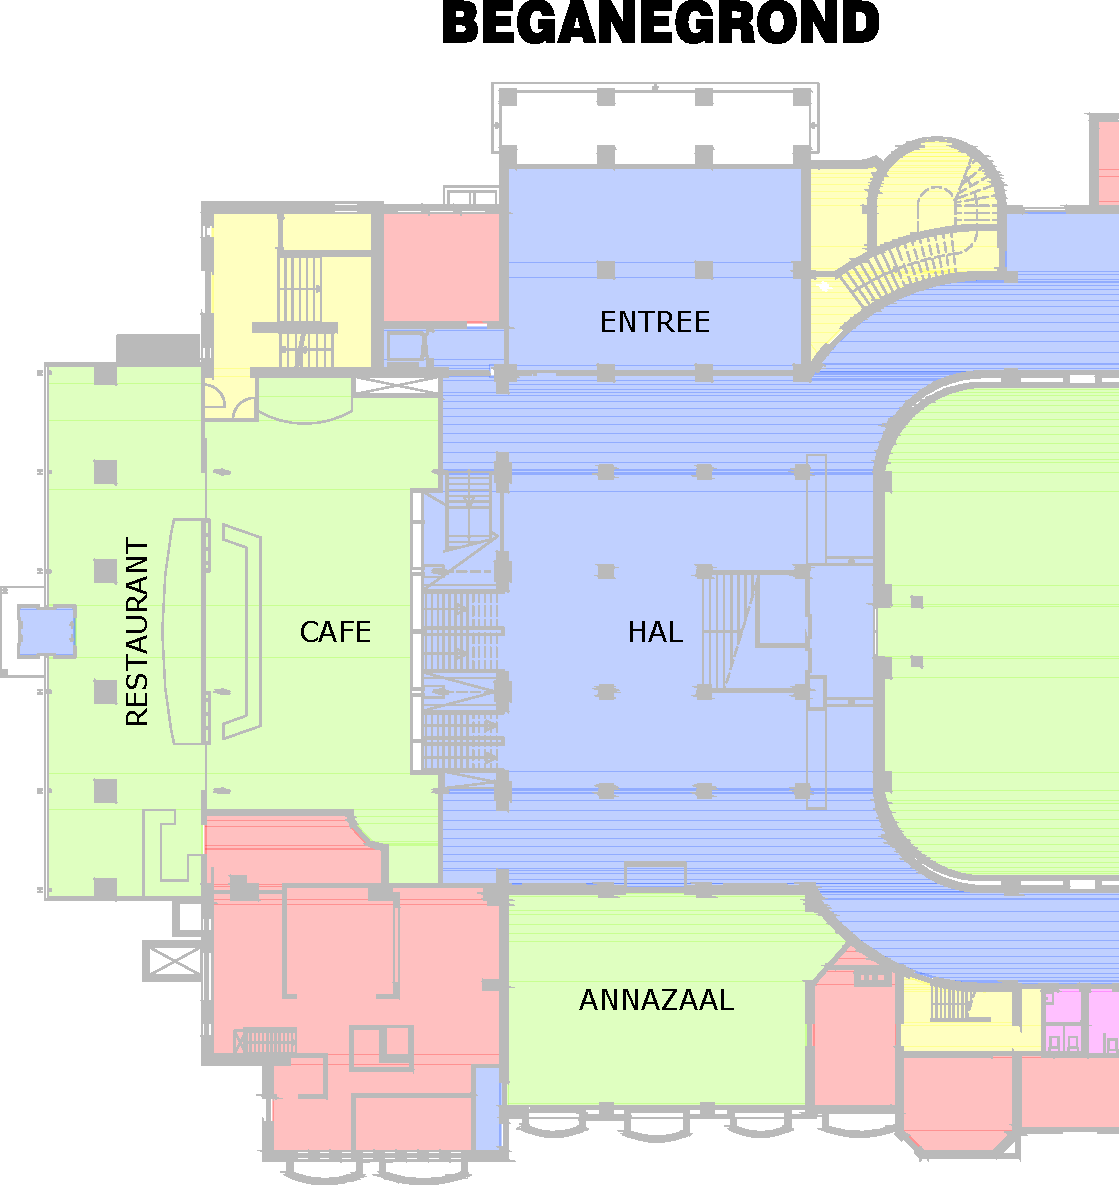
\includegraphics[width=.85\textwidth]{beneden3} \hspace{1cm}
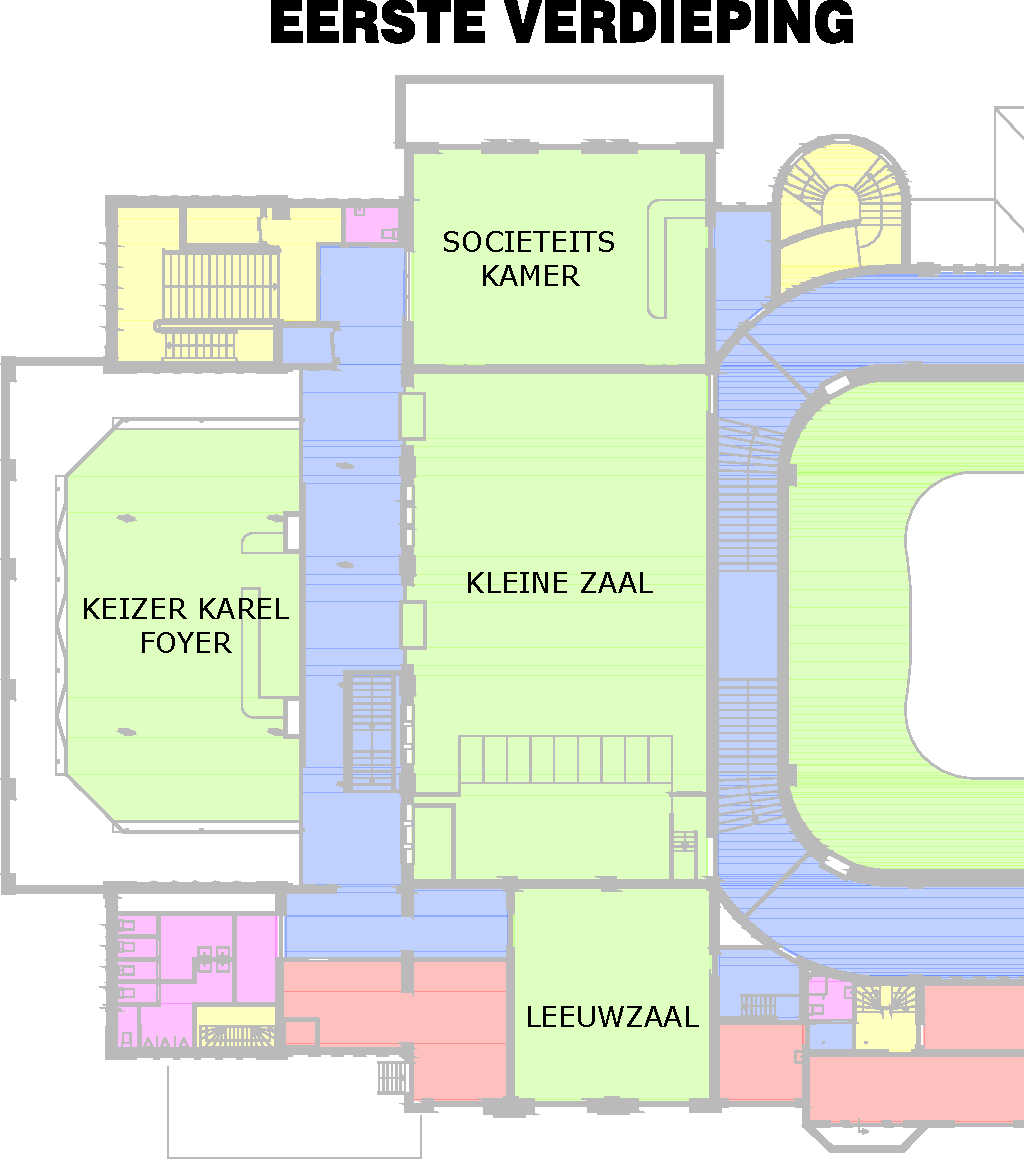
\includegraphics[width=.75\textwidth]{boven3}
\end{landscape}

\newpage

\notes[10pt]{15}{\textwidth}

\newpage

\notes[10pt]{15}{\textwidth}

\newpage

\notes[10pt]{15}{\textwidth}


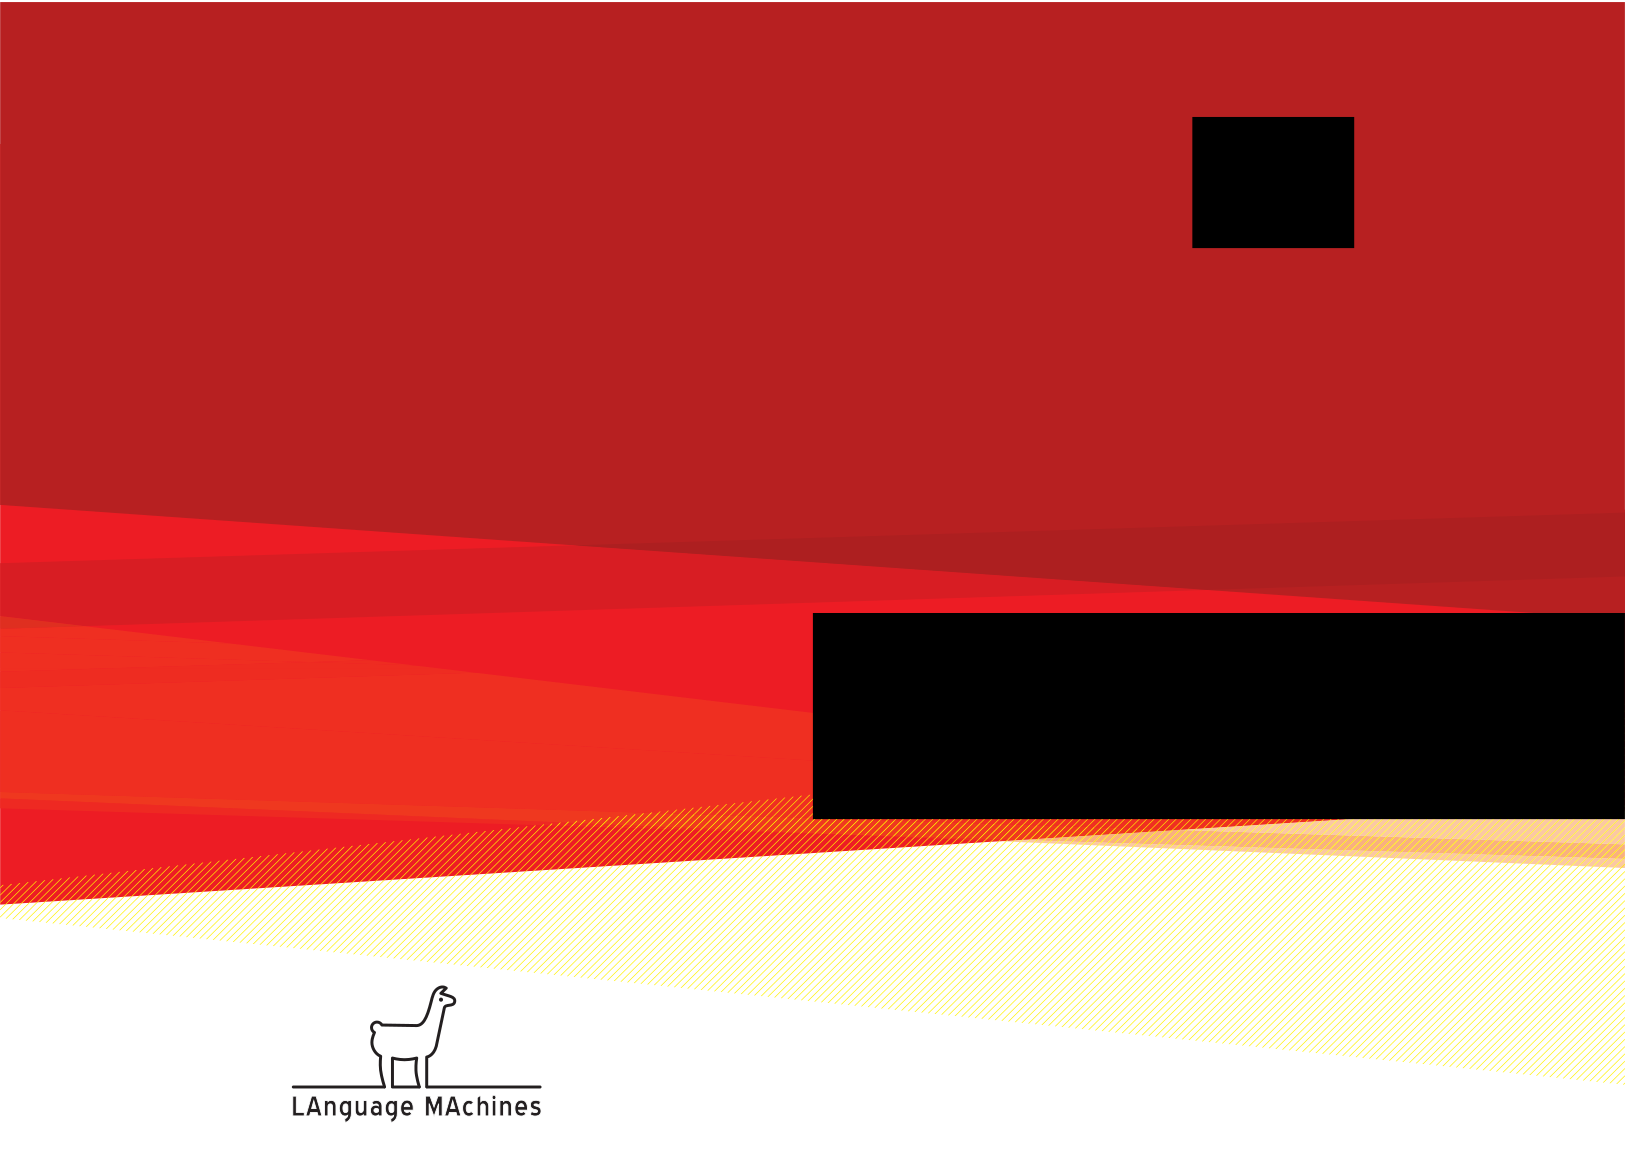
\includepdf[clip, trim=0.0cm 0cm 21.5cm 0.0cm, width=1.00\paperwidth]{front}
\end{document}
